%%%%%%%%%%%%%%%%%%%%
%% 04-RESULTS %%
%%%%%%%%%%%%%%%%%%%%
\clearpage\section{Implementation and results}

In this chapter we will explain the different use cases that our framework provides along with the programs captures of the tools explained in chapter 3.

We will explain one workflow for each tool.

\subsection{lxce}
For the first workflow, we will explain how to initialize the command and manage some containers configurations.

In specific we will:
\begin{itemize}
	\item{Initialize the command}
	\item{Create some containers}
	\item{Change linux distributions for containers}
	\item{Delete some containers}
	\item{Add and delete proxies on containers}
	\item{Delete the command and configurations}
\end{itemize}

%%% INITIALIZE COMMAND %%%
\textbf{Initialize the command}
The first thing we have to do is initialize the command in order to generate the default configurations files and select different parameters.

\begin{minted}[bgcolor=background]{console}
root@oscar-vm: # lxce init
? lxce.conf: Select hypervisor hostname: localhost
? lxce.conf: Select ssh suffix: oscar-vm
? lxce.conf: Select vnc server: localhost
? lxce.conf: Select vnc port: 5901
? lxce.conf: Select data location [full path]: /datasdd
? Want to add another data location (just hit enter for YES)? No
? container.default: Select containers base: ubuntu:20.04
? container.default: Select default container location: /datasdd
[] Good!
root@oscar-vm: #
\end{minted}

%%% CREATE SOME CONTAINERS %%%
\newpage
\textbf{Create containers}
Then we can create 3 containers with different alias in the domain test with:
\begin{minted}[bgcolor=background]{console}
root@oscar-vm: # lxce launch -r 3 -d test -a alice bob peter 
[*] --------------------------------------------------------------
[*] Checking ...
[*] Initialized
[*] Initialized: ok!
[*] Access
[*] Access: ok!
[*] Checks: ok!
[*] --------------------------------------------------------------
[*] Launching container with managing-harlequin
[**] launching ...
[**] waiting for container...
[**] Getting user
[**] Getting user: ubuntu !!
[**] Password created: fa89a2eaca
[**] launching: ok!
[**] creating configurations
[**] creating configurations: ok!
[**] read only directories
[**] added data-test shared folder
[**] added data-managing-harlequin shared folder
[**] read only directories: ok!
[**] adding proxies
[**] added proxy-ssh
[**] added proxy-test
[**] adding proxies: ok!
[**] dns resolution: managing-harlequin.lxd -> 10.10.1.171
[] Launching container with managing-harlequin
[*] Launching container with excited-amethyst
[] Launching container with excited-amethyst
[*] Launching container with coloured-purple
[] Launching container with coloured-purple
[*] --------------------------------------------------------------
[*] Success!!
\end{minted}
Where we can see the containers created, along with their properties, with:

\begin{figure}[H]
\label{fig:lxce list}
\centering
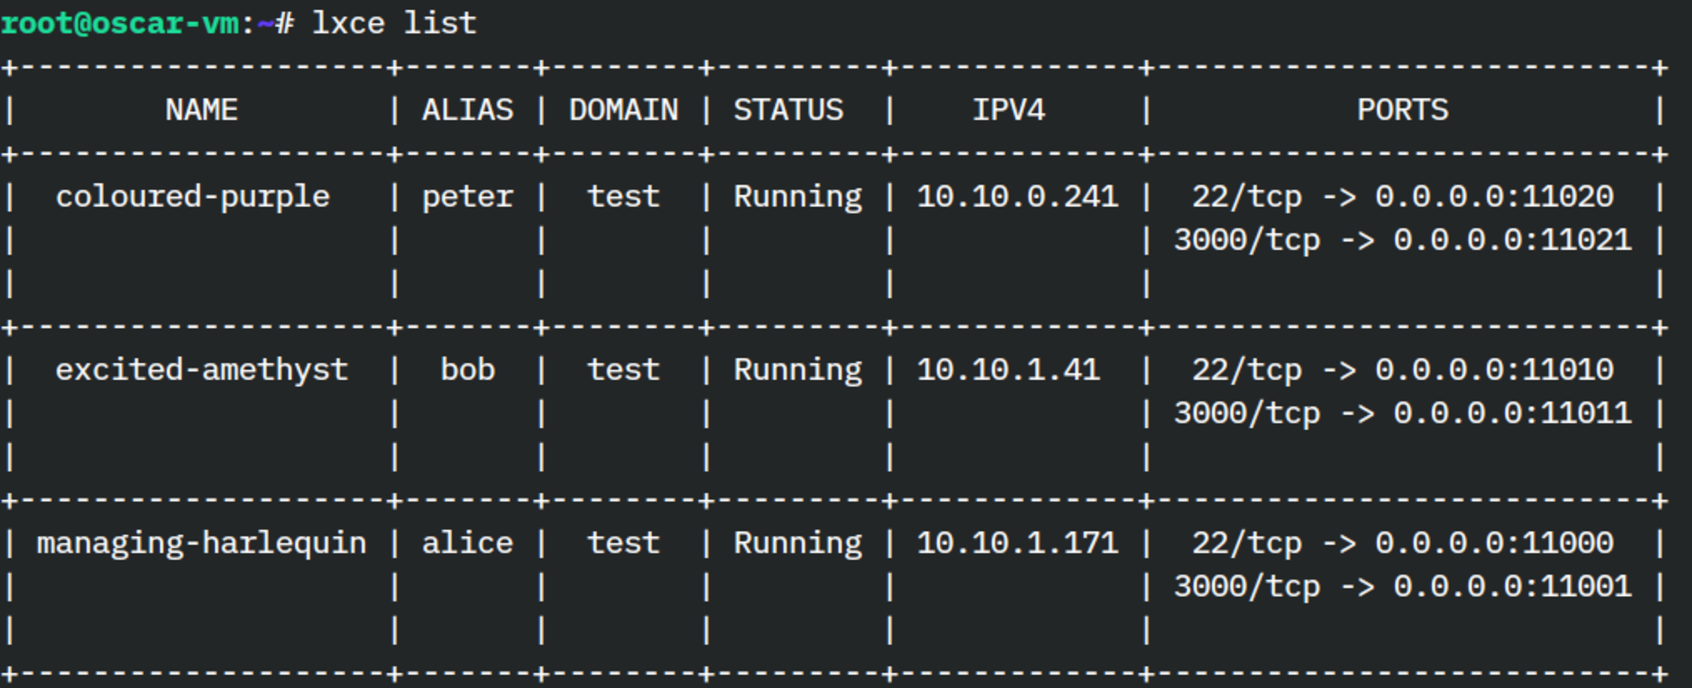
\includegraphics[width=\textwidth]{img/04/lxce-list.pdf}
\caption[Prototype setup]{\footnotesize{lxce list.}}
\end{figure}


%%% CHANGE CONTAINER BASES %%%
\textbf{Change container base}
We have set up all the containers to be run with an ubuntu:20.04 base, but if we we would like to change one container (peter for example) to use ubuntu:18.04 instead we could do it by:
\begin{minted}[bgcolor=background,breaklines]{console}
root@oscar-vm: # lxce rebase -d test -a peter -b ubuntu:18.04
? Do you want to rebase coloured-purple container within test with ubuntu:18.04? Yes
[*] Rebasing coloured-purple
[**] Removing coloured-purple
[**] launching container with base: ubuntu:18.04 ...
[**] waiting for container
[**] Getting user
[**] Getting user: ubuntu !!
[**] added proxy-ssh
[**] added proxy-test
[**] added data-ubuntu
[**] added data-test
[**] dns resolution: coloured-purple.lxd -> 10.10.0.168
[] Rebasing coloured-purple
\end{minted}
where all the properties of the container will remain the same.

So then we would have the following:
\begin{minted}[bgcolor=background]{console}
root@oscar-vm: # lxce list -c nadb
+--------------------+-------+--------+--------------+
|        NAME        | ALIAS | DOMAIN |     BASE     |
+--------------------+-------+--------+--------------+
|  coloured-purple   | peter |  test  | ubuntu:18.04 |
+--------------------+-------+--------+--------------+
|  excited-amethyst  |  bob  |  test  | ubuntu:20.04 |
+--------------------+-------+--------+--------------+
| managing-harlequin | alice |  test  | ubuntu:20.04 |
+--------------------+-------+--------+--------------+
\end{minted}

%%% DELETE SOME CONTAINERS %%%
\textbf{Delete containers}
Now if we want to delete a specific container, it's configuration and shared folder:

\begin{minted}[bgcolor=background, breaklines]{console}
root@oscar-vm: # lxce delete -d test -a alice
[*] Init: ok!
[*] Permission checked
? Do you want to delete managing-harlequin? Yes
[**] Removing managing-harlequin
\end{minted}

%%% UNINSTALL COMMAND %%%
\textbf{Uninstall command}
Finally, if we want to uninstall the command (i.e: remove all containers, configurations files and shared locations folders) we simply:
\begin{minted}[bgcolor=background, breaklines]{console}
root@oscar-vm: # lxce uninstall
[*] Init: ok!
[*] Permission checked
? Do you want to uninstall the lxce command and all it's configurations? Yes
[*] Deleting and stopping current containers
[**] Removing coloured-purple
[**] Removing excited-amethyst
[*] Delete /etc/lxce/
\end{minted}

\subsection{lxce-admin}
The second workflow will consist in how to use the "lxce-admin" tool to manage and existing host with the lxce command installed.

For this example we will do it everything in local but the same applies for external machines with remote access.

But before starting typing commands in the admin host, we must set up the following in each of the hosts with lxce installed:
\begin{itemize}
	\item{Install lxce}
	\item{Init lxce and configure container bases with graphical support for enabling VNC access}
	\item{Configure public key access to host}
	\item{Set up a localhost VNC server listening according to the lxce configuration file}
\end{itemize}

%%% ADD HOST %%%
\textbf{Add host}
The first thing that we must do is to add a remote host:
\begin{minted}[bgcolor=background, breaklines]{console}
root@oscar-vm: # lxce-admin config add
? Select host (ssh config): oscar-vm
? Select hostname: localhost
? Select ssh port: 22
? Select private key location [full path]: /home/oscar/.ssh/localhost_oscar
[*] Updating files
[**] Updating passwords
[*] Updating files: ok
\end{minted}

\begin{minted}[bgcolor=background, breaklines]{console}
root@oscar-vm: # lxce-admin config list
+----------+---------+------------+
|   HOST   | DOMAINS | CONTAINERS |
+----------+---------+------------+
| oscar-vm |    1    |     3      |
+----------+---------+------------+
\end{minted}

\newpage
\textbf{Test SSH}
Once set up the host, we have already access to the ssh configuration file of each container.

We can test it by ssh [host.domain.containerName/containerAlias]:
\begin{minted}[bgcolor=background, breaklines]{console}
root@oscar-vm: # ssh oscar-vm.google.itchy-bronze
ubuntu@192.168.122.118's password:

The programs included with the Ubuntu system are free software;
the exact distribution terms for each program are described in the
individual files in /usr/share/doc/*/copyright.

Ubuntu comes with ABSOLUTELY NO WARRANTY, to the extent permitted by
applicable law.

To run a command as administrator (user "root"), use "sudo <command>".
See "man sudo_root" for details.

ubuntu@itchy-bronze:~$
\end{minted}

\textbf{VNC}
Another service that is available is VNC access to every container.

For connecting to the container through VNC we can use two methods:
\begin{itemize}
	\item{\textbf{lxce-admin vnc}: will open a normal VNC client}
\begin{minted}[bgcolor=background, breaklines]{console}
root@oscar-vm: # lxce-admin vnc --host oscar-vm -d google -n real-black --scale 1
\end{minted}
	\item{\textbf{lxce-admin remmina}: will open remmina (VNC client). The advantage is that remmina is able to use system passwords saved in the computer chain generated by the command, so we won't have to type the ssh password not the vnc password}
\begin{minted}[bgcolor=background, breaklines]{console}
root@oscar-vm: # lxce-admin remmina --host oscar-vm -d google -n real-black
\end{minted}
\end{itemize}

\TODO{put commands descriptions each}

\subsection{web-admin}
For configuring the web-admin web app we should:
\begin{itemize}
	\item{Start the web application in an admin host}
	\item{Start the express server in each of the hosts with lxce installed in order to serve the corresponding API}
\end{itemize}

Once everything is set up, the main page of the web application is the following:
\begin{figure}[H]
\label{fig:web-admin}
\centering
\frame{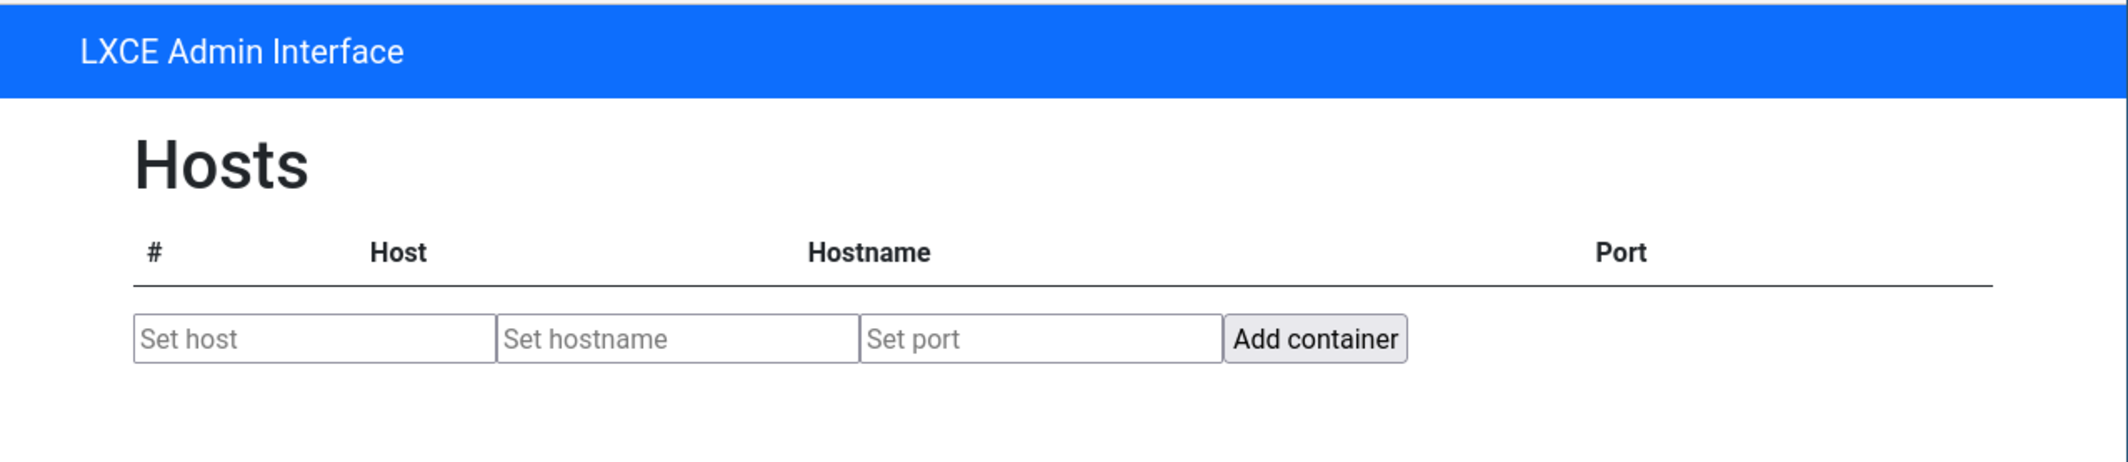
\includegraphics[width=\textwidth]{img/04/web-admin-first.pdf}}
\caption[Prototype setup]{\footnotesize{lxce list.}}
\end{figure}

Where we can add a host:
\begin{figure}[H]
\label{fig:lxce list}
\centering
\frame{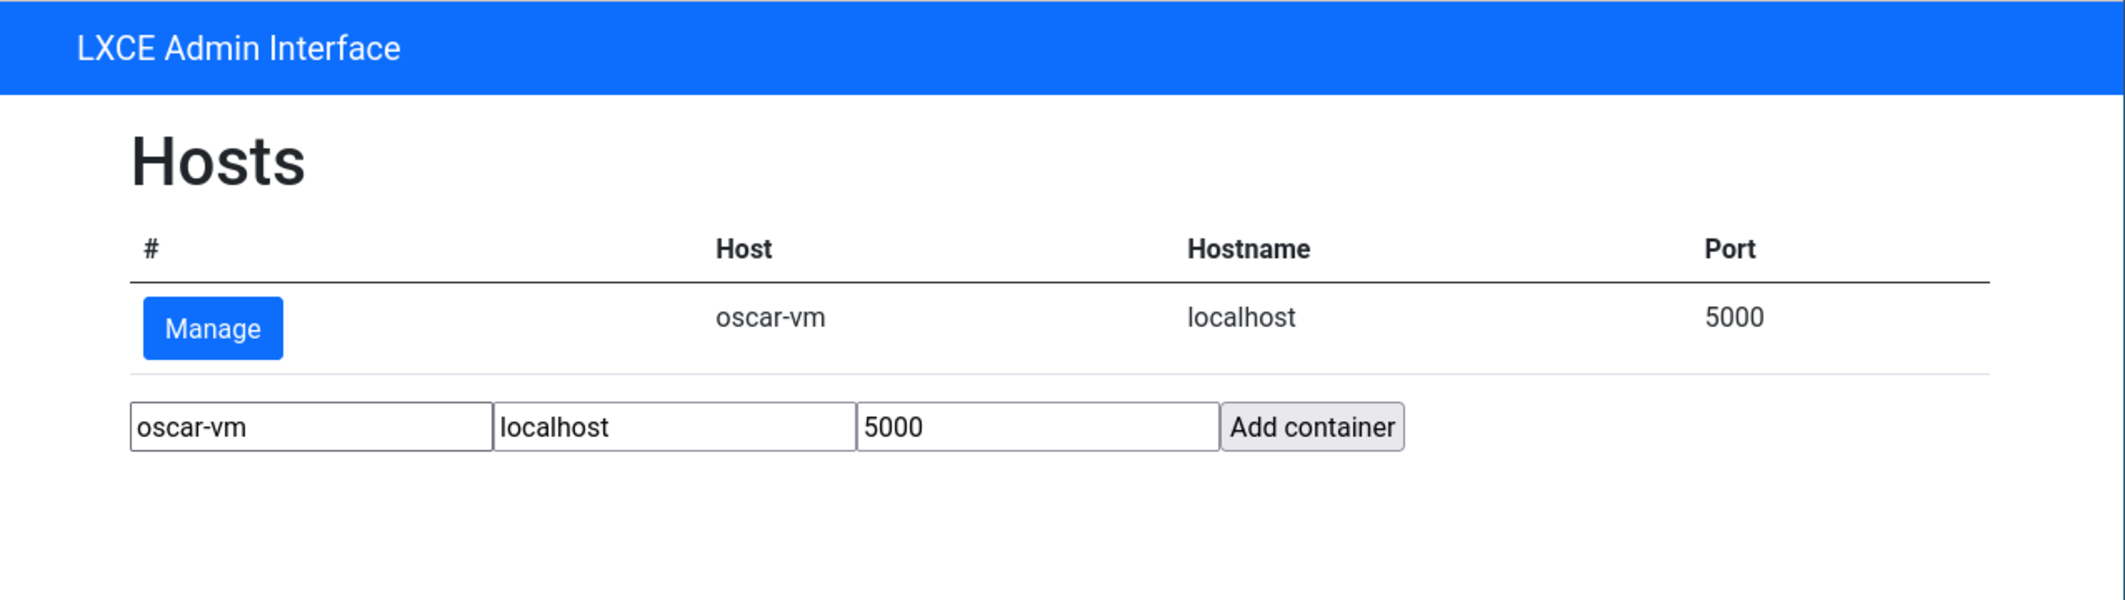
\includegraphics[width=\textwidth]{img/04/web-admin-second.pdf}}
\caption[Prototype setup]{\footnotesize{lxce list.}}
\end{figure}

\newpage
And view the container for each host along with the container properties:
\begin{figure}[H]
\label{fig:lxce list}
\centering
\frame{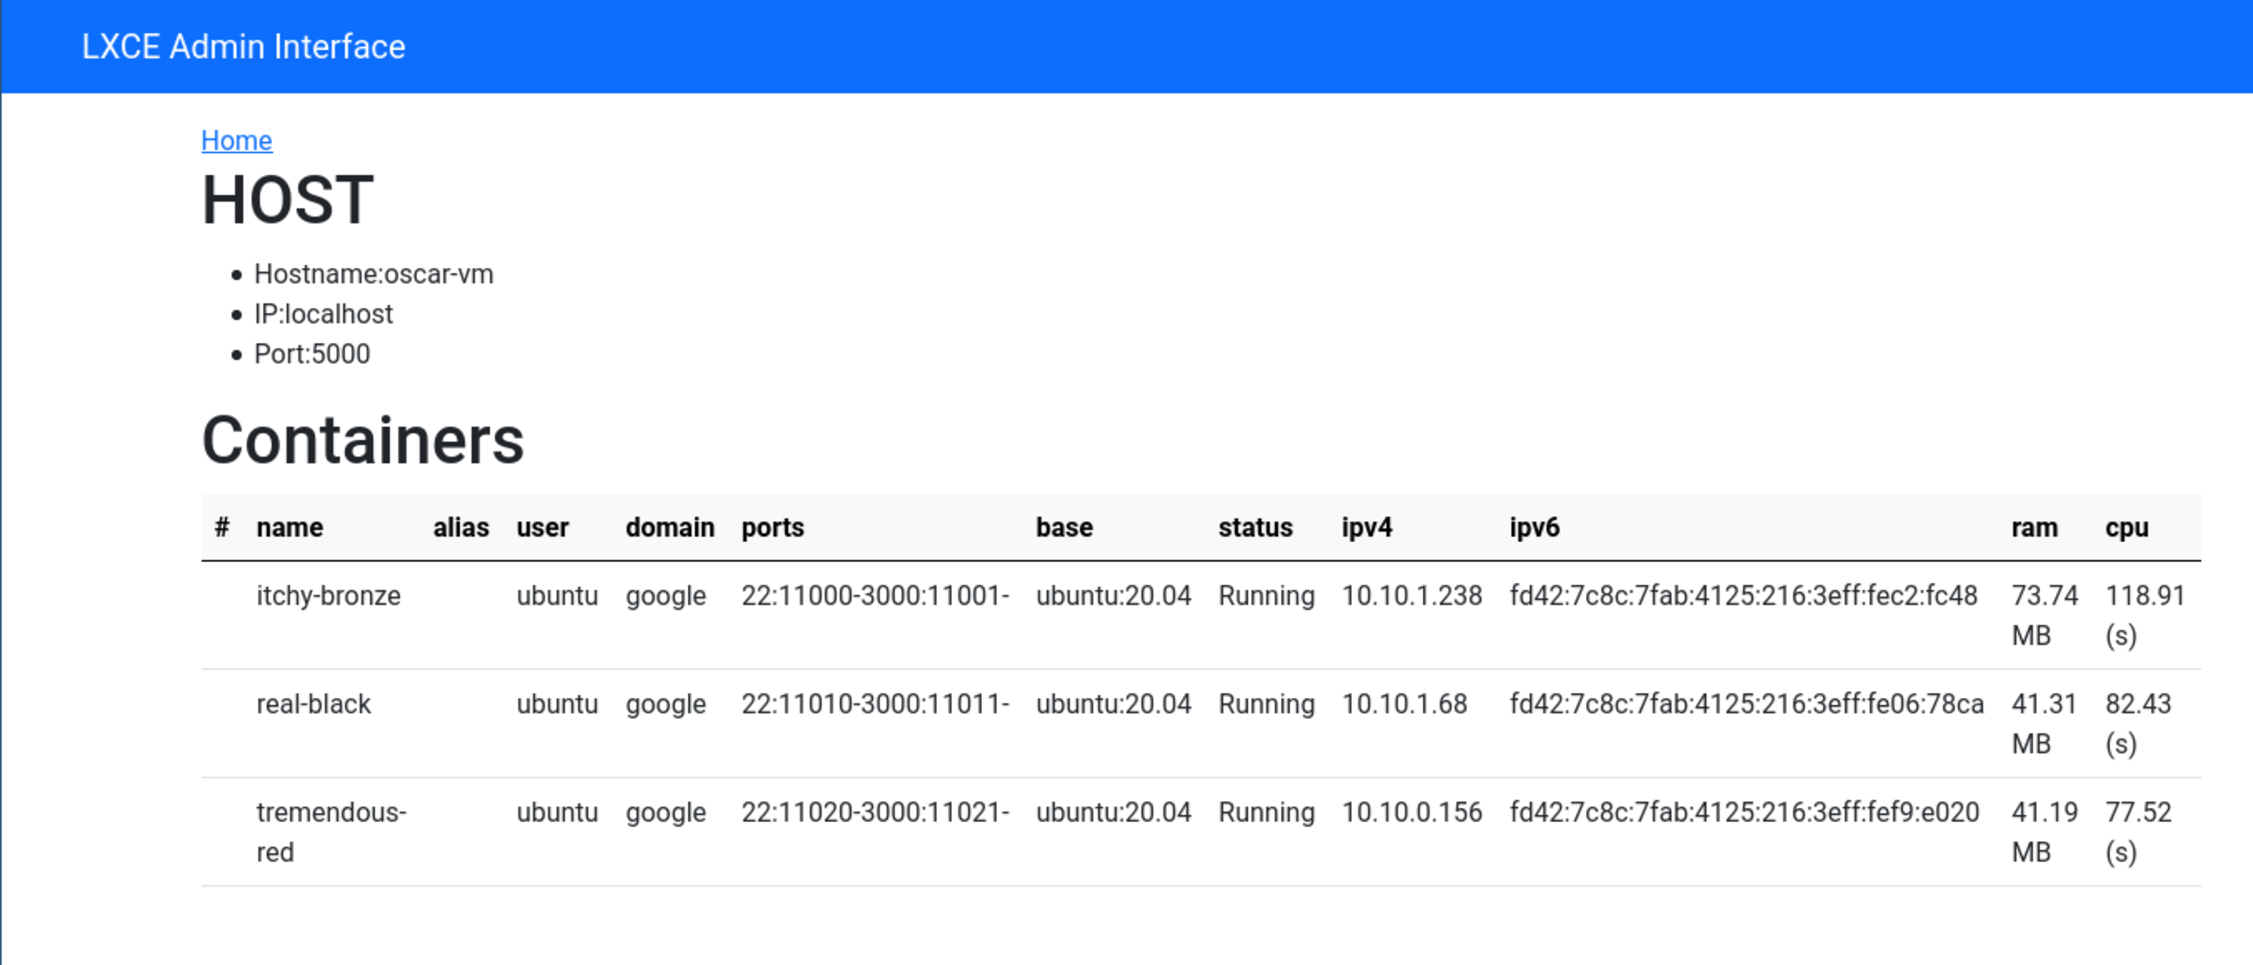
\includegraphics[width=\textwidth]{img/04/web-admin-third.pdf}}
\caption[Prototype setup]{\footnotesize{lxce list.}}
\end{figure}


